\chapter{VALIDAÇÃO DO CÓDIGO NÚMERICO}
\label{validacao}
\section{\textbf{Introdução}}
Neste capítulo serão apresentados as comparações realizadas entre os resultados numéricos obtidos para x casos amplamente conhecidos na literatura e a solução analítica unidimensional dos mesmos.
Como a solução numérica é obtida para problemas bidimensionais, é preciso pegar uma seção transversal do domínio e interpolar  resultado, produzindo, assim, uma aproximação.
Dessa forma, a quantificação do erro relativo médio se faz necessária, com o objetivo de apresentar a acurácia do código numérico. O erro relativo entre a solução numérica e a solução analítica é calculado pela equação \eqref{error_eq}:
\begin{equation}
    er_i = \frac{|(val_a)_i - (val_n)_i|}{(val_a)_i}
    \label{error_eq} 
\end{equation}
onde $(val_a)_i$ é o valor encontrado pela solução analítica e $(val_n)_i$ é o valor encontrado pela solução numérica, ambos encontrados no ponto $i$.

São calculados também a média e o desvio padrão dos erros relativos pelas equações \eqref{error_mean} e \eqref{error_mean}, respectivamente:
\begin{equation}
    er_{mean} = \frac{1}{N}\sum_{i=0}^{N} er_i
    \label{error_mean}
\end{equation}
\begin{equation}
    er_{std} = \sqrt{\frac{1}{N}\sum_{i=0}^{N} (er_i-er_{mean})^2}
    \label{error_std} 
\end{equation}

As validações foram organizadas em três seções que representam diferentes etapas da implementação do modelo matemático, sendo assim espera-se mostrar a aplicabilidade do código numérico desenvolvido, além do histórico de aprendizado obtido.
Na seção \ref{sec_solidos}, os problemas de transferência de calor em sólidos com condutividade termica constante são apresentados.
Os casos propostos nesta seção buscam confirmar a importação correta da malha e a montagem das matrizes globais, como também a aplicação das condições de contorno de Dirichlet e de Neumann.

Já na seção \ref{sec_fluidos}, os problemas com o termo convectivo presente são analisados.
Foi considerado o fluido como incompressível e newtoniano, dessa forma a equação de Navier-Stokes pode ser aplicada segundo a formulação corrente-vorticidade.
A estrutura do algoritmo de solução nos casos propostos dessa seção é a mesma utilizada na resolução do problema proposto neste trabalho.
Dessa forma, podemos confirmar a correta aplicação das condições de contorno da vorticidade que deve ser calculada em cada passo de tempo.
%No final da seção, apresentamos um caso onde o número de Reynolds é aumentado até as oscilações numéricas serem visualizadas e, assim, verificar o limite de aplicabilidade do código.

Finalmente, na seção \ref{sec_particulas}, é apresentado os clássicos casos de dinâmica em partículas com o intuito de validar as forças de gravidade, arrasto e sustentação isoladamente e, com isso, possibilitar uma a correção pontual no modelo quando
necessário, alem de permitir observar com maior precisão a influência da atuação que cada uma das força faz sobre a partícula.

Para casos com variáveis temporais, foi utilizado um critério de parada de $10^{-5}$ de variação de valores entre dois intervalos de tempo consecutivos.
Desta maneira espera-se que o sistema já tenha entrado na situação de convergência e esteja próximo o suficiente de seus valores finais.
Isto foi feito para poupar tempo de computação, para casos que possuem um limite de tempo elevado e convergem rapidamente, fazendo com que o código continuasse desnecessariamente.

A execução do código e a computação dos resultados foram realizados em um computador de uso pessoal com as seguintes especificações:
\begin{itemize}
    \item Dell Latitude E6410 com processador Intel® Core™ i5 CPU M 520 2.40GHz com 4 núcloes e 4Gb de memória RAM.
          O sistema operacional ubuntu 16.04 LTS e compilador Python 3.5.
\end{itemize}


%---------------------------------------------------------------------------------------------Validação de sólidos
\section{\textbf{Validações de Problemas em Sólidos}}
\label{sec_solidos}
%---------------------------------------------------------------------------------------------Primeiro Exemplo
\subsection{\textbf{Equação de Laplace com Condições de Contorno de Dirichlet}}
\label{sec_laplace_dir}
O problema de troca de calor em uma placa é um dos exemplos clássicos utilizados para estudar as equações de transmissão de calor em sólidos. O mais simples destes é uma barra unidimensional com condutividade térmica constante e sem geração de calor onde a temperatura é conhecida nas extremidades.
Como a malha do código foi desenvolvida para solução de problemas bidimensionais, cria-se um problema bidimensional com condições de contorno equivalentes e extrai-se uma seção para que se possa comparar os resultados.

A equação de governo deste fenômeno é conhecida como a equação de Laplace \eqref{laplace_d_perm_eq} para sólidos em estado permanente e é apresentada a seguir:
\begin{equation}
    \nabla^2 T = 0
    \label{laplace_d_perm_eq} 
\end{equation}
onde T é a temperatura na placa e $\nabla^2$ é o operador diferencial conhecido como laplaciano.

E a solução analítica do problema unidimensional associado é:
\begin{equation}
    T(x) = \dfrac{T_L-T_0}{L} x + T_0
    \label{laplace_d_sol}
\end{equation}
onde $L$ é o comprimento da barra, $T_0$ e $T_L$ são, respectivamente, os valores da temperatura em $x=0$ e $x=L$.

As condições de contorno e o dominio bidimensional utilizados na simulação são apresentados na \ref{laplace_d_bc}. A condição de fluxo de calor $\dfrac{\partial T}{\partial n}$ nulo significa que nenhuma condição é imposta no contorno.

\begin{figure}[H]
    \centering
    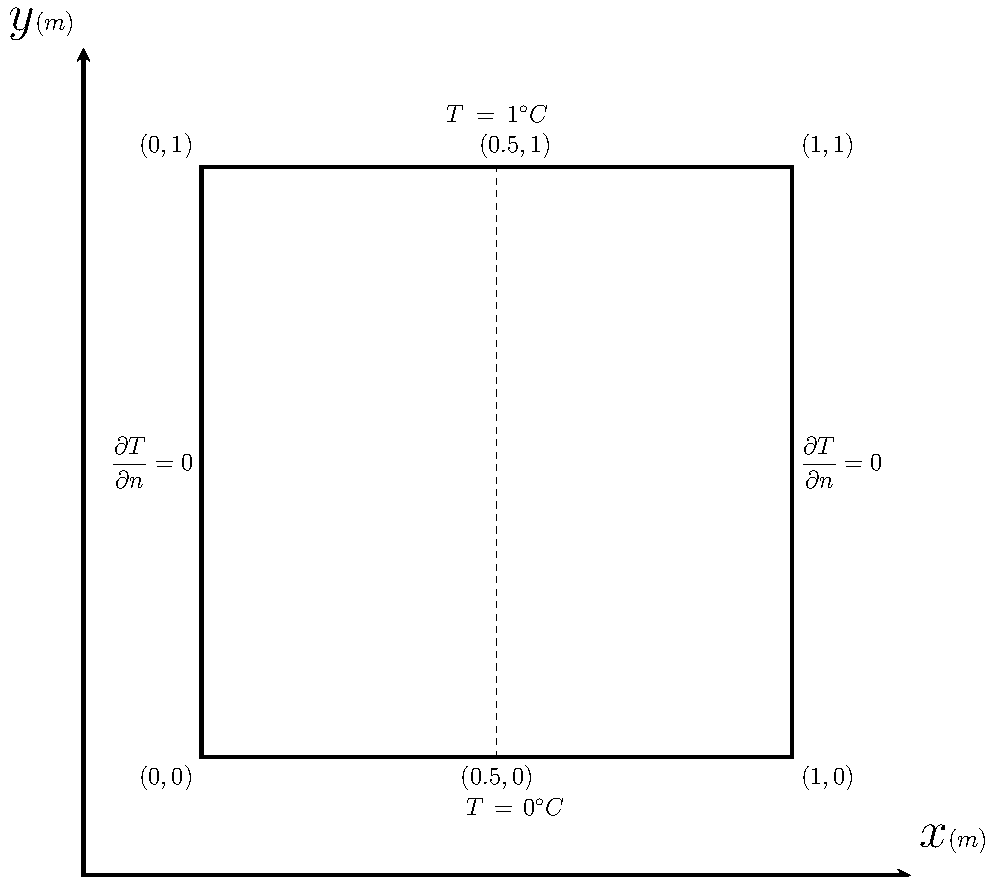
\includegraphics[width=.7\linewidth]{figures/laplace_dirichlet_boundary_conditions.pdf}
    \caption{Condições de contorno da placa para o problema de Laplace \ref{sec_laplace_dir}.}
    \label{laplace_d_bc}
\end{figure}

O dominio foi discretizado utilizando uma malha triangular linear não estruturada com 768 elementos e 417 nós.
A malha foi criada pelo o software GMSH como proposto por \cite{gmsh} e importada ao código numérico.
A \ref{laplace_d_3d} apresenta o campo de temperatura, onde os eixos $x$ e $y$ representam o dominio e o eixo $z$ é a distribuição de temperatura, e que é possível observar que o campo de temperatura possui um perfil linear variando de 0 (cor azul) a 1 (cor vermelha).
\begin{figure}[H]
    \centering
    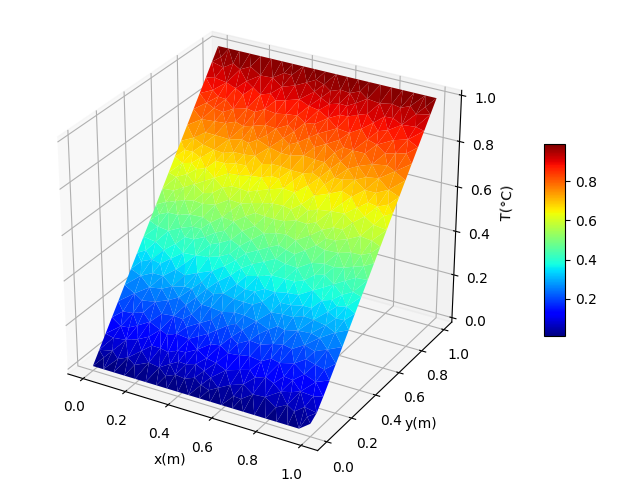
\includegraphics[width=.7\linewidth]{figures/laplace_dirichlet_permanent_3d.png}
    \caption{Distribuição de temperaturas na placa da solução permanente da equação de Laplace \ref{sec_laplace_dir}.}
    \label{laplace_d_3d}
\end{figure}

A comparação entre os resultados da solução analítica \eqref{laplace_d_sol} e a solução numerica, para a seção $x=0.5m$, é apresentada na \ref{laplace_d_perm_comp}, onde é possível observar que ambas possuem o mesmo perfil.
Essa proximidade é quantificada pelo erro relativo médio que foi de $0.1136\%$ e com desvio padrão de $0.0008\%$
\begin{figure}[H]
    \centering
    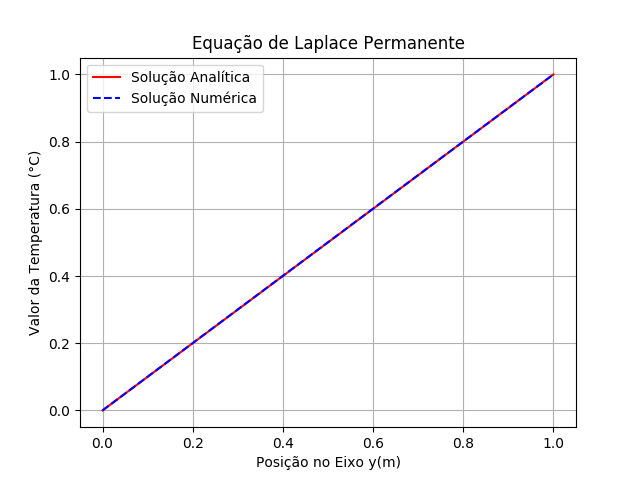
\includegraphics[width=.7\linewidth]{figures/laplace_dirichlet_permanent_comparison.png}
    \caption{Comparação de resultado das soluções númerica e analítica do caso de transporte de temperatura em sólidos no regime permanente.}
    \label{laplace_d_perm_comp}
\end{figure}

Ao solucionar o mesmo problema introduzindo o termo transiente na equação de governo \ref{laplace_d_perm_eq}, pode-se verificar a evolução de comportamento da temperatura ao longo do tempo.
Dessa forma, a equação que representa este caso é:
\begin{equation}
    \dfrac{\partial T}{\partial t} + k\nabla^2 T = 0
    \label{laplace_d_trans_eq} 
\end{equation}
onde $k$ é o coeficiente de condutividade térmica da placa e $t$ é a variável temporal.

Porém, ao longo dos passos de tempo, a solução se aproxima de um problema permanente, portanto pode-se fazer a comparação dos resultados obtidos neste exemplo com os valores da solução analítica \eqref{laplace_d_sol}, tomando-se que $t\rightarrow \infty$.
As condições iniciais $t=0s$ atribuídas aos nós sem condição de contorno foram de um valor inicial de $0^{\circ}C$.
A \ref{laplace_d_trans_comp} apresenta a evolução do campo de temperaturas em função do tempo.
É possível observar que a solução numérica converge para a solução analítica formando um perfil linear.
O erro relativo médio calculado para este caso foi de $0.1092\%$ e com desvio padrão de $0.0008\%$.
\begin{figure}[H]
    \centering
    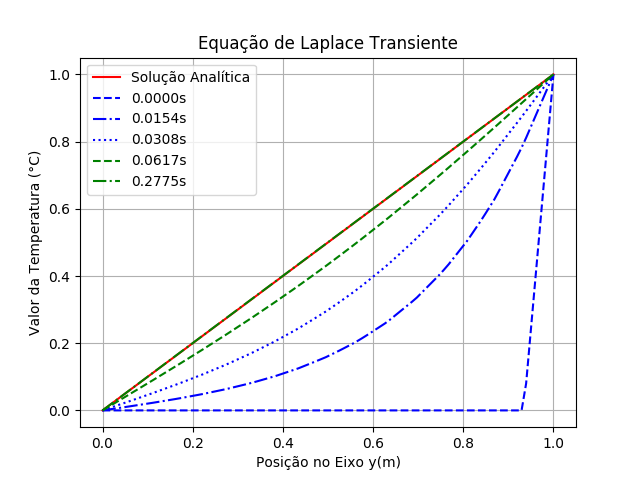
\includegraphics[width=.7\linewidth]{figures/laplace_dirichlet_transient_comparison.png}
    \caption{Comparação de resultado das soluções númerica e analítica de transporte em sólidos no regime transiente.}
    \label{laplace_d_trans_comp}
\end{figure}


%---------------------------------------------------------------------------------------------Segundo Exemplo
\subsection{\textbf{Equação de Poisson com Condições de Contorno de Dirichlet}}
\label{sec_poisson_dir}
Neste problema busca-se estudar o comportamento de uma placa com geração de calor em seu domínio e temperaturas fixas nas laterais.
Novamente, para permitir a comparação de resultados, é extraída uma seção da placa para observar os resultados como um problema unidimensional.

A equação que governa este caso é denomidada equação de Poisson \eqref{poisson_d_perm_eq}, tomada para um problema permanente, ou seja sem variação no tempo.
\begin{equation}
    -k\nabla^2 T = Q
    \label{poisson_d_perm_eq} 
\end{equation}
onde $Q$ é a geração de calor na placa.

A solução analítica para o caso de uma barra unidimensional é apresentada embaixo:
\begin{equation}
    T(x) = \dfrac{Q}{2k}\left(-x^2 + L x\right) + \dfrac{T_L-T_0}{L} x + T_0
    \label{poisson_d_sol} 
\end{equation}

As condições de contorno e o dominio bidimensional utilizados na simulação são apresentados na \ref{poisson_d_bc}.
A geração de calor utilizada foi de $Q = 40W/m^3$ e a condutividade termica foi de $k=5 W/m^{\circ}C$.
\begin{figure}[H]
    \centering
    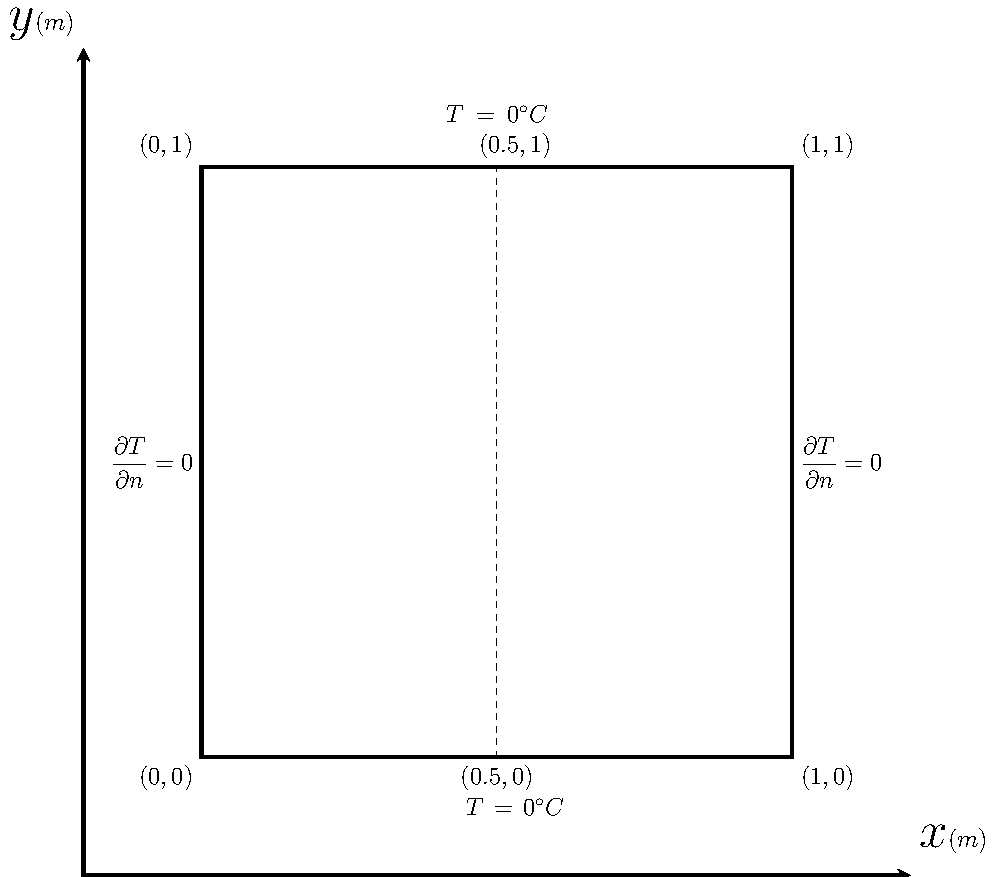
\includegraphics[width=.7\linewidth]{figures/poisson_dirichlet_boundary_conditions.pdf}
    \caption{Condições de contorno da placa para o problema de Poisson \ref{sec_poisson_dir}.}
    \label{poisson_d_bc}
\end{figure}

Novamente, foi utilizada uma malha triangular linear não estruturada com 768 elementos e 417 nós.
A \ref{poisson_d_3d} apresenta o campo de temperatura, onde os eixos $x$ e $y$ representam o dominio e o eixo $z$ é a distribuição de temperatura, onde é possível observar que o campo de temperatura possui um perfil parabólico variando de 0 (cor azul) a 1 (cor vermelha).
\begin{figure}[H]
    \centering
    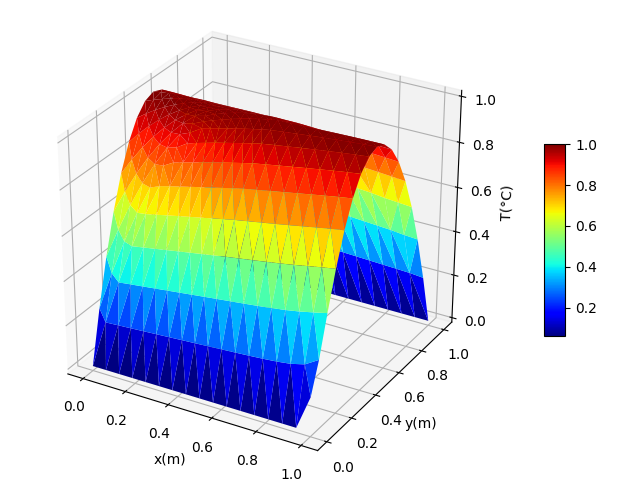
\includegraphics[width=.7\linewidth]{figures/poisson_dirichlet_permanent_3d.png}
    \caption{Distribuição de temperaturas na placa da solução do problema permanente de Poisson \ref{sec_poisson_dir}.}
    \label{poisson_d_3d}
\end{figure}

A comparação entre os resultados da solução analítica \eqref{poisson_d_sol} e a solução numerica, para a seção $x=0.5m$, é apresentada na \ref{poisson_d_perm_comp}, onde é possível observar que ambas possuem o mesmo perfil.
Essa proximidade é quantificada pelo erro relativo médio que foi de $0.323\%$ e com desvio padrão de $0.0101\%$.
\begin{figure}[H]
    \centering
    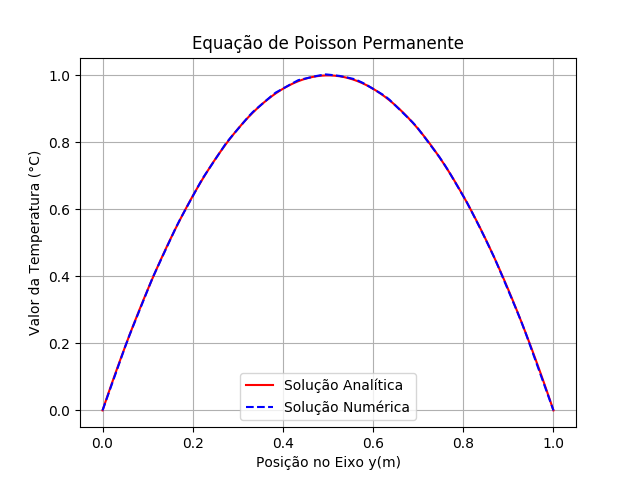
\includegraphics[width=.7\linewidth]{figures/poisson_dirichlet_permanent_comparison.png}
    \caption{Comparação de resultado das soluções númerica e analítica do problema de transporte de temperatura em sólidos no regime permanente com geração de calor.}
    \label{poisson_d_perm_comp}
\end{figure}

A seguir, é apresentado o resultado com termo transiente $\dfrac{\partial T}{\partial t}$ tendendo a um estado permanente.
As condições iniciais $t=0s$ atribuídas aos pontos sem condição de contorno foram de um valor inicial de $0^{\circ}C$.
A \ref{poisson_d_trans_comp} apresenta a evolução do campo de temperaturas em função do tempo.
É possível observar que a solução numérica converge para a solução analítica formando um perfil parabólico.
O erro relativo médio calculado para este caso foi de $0.325\%$ e com desvio padrão de $0.0101\%$.
\begin{figure}[H]
    \centering
    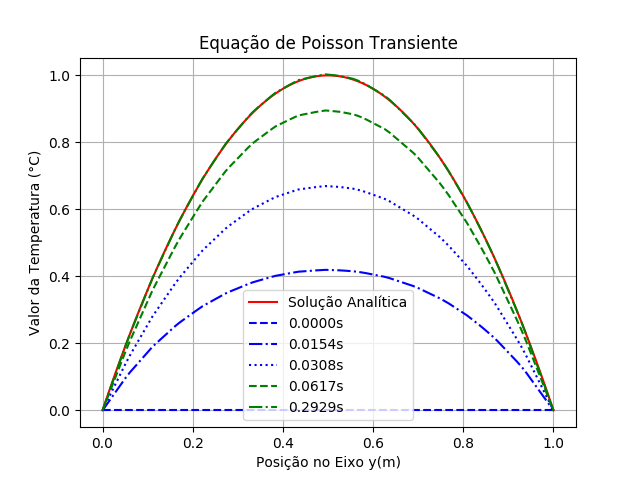
\includegraphics[width=.7\linewidth]{figures/poisson_dirichlet_transient_comparison.png}
    \caption{Comparação de resultado das soluções númerica e analítica do problema de trasnporte de temperatura em sólidos no regime transiente com geração de calor.}
    \label{poisson_d_trans_comp}
\end{figure}

%---------------------------------------------------------------------------------------------Terceiro Exemplo
\subsection{\textbf{Equação de Poisson com Condições de Contorno de Dirichlet e Neumann}}
\label{sec_poisson_neu}
Este caso foi escolhido para validar a solução de problemas com condições de contorno de Neumann.
Trata-se de uma placa com temperatura fixa em uma das paredes e no lado oposto é defido um valor para o fluxo de calor presente.
Toma-se uma seção da placa para observar os resultados e compará-los com um problema unidimensional de uma barra com as mesmas condições presentes.

A equação de governo é novamente a equação de Poisson \eqref{poisson_d_perm_eq}, e sua solução analítica para uma barra unidimensional é dada por:
\begin{equation}
    T(x) = \dfrac{Q}{k}\left(\dfrac{-x^2}{2} + L x\right) - \dfrac{q}{k} x + T_0
    \label{poisson_n_sol} 
\end{equation}
onde $q$ é o fluxo de calor na extremidade $x=L$.

As condições de contorno e o dominio bidimensional utilizados na simulação são apresentados na \ref{poisson_n_bc}.
A geração de calor utilizada foi de $Q = -7W/m^3$, a condutividade termica foi de $k=5 W/m^{\circ}C$ e o fluxo de calor foi de $q = -5 W/m^2$.
\begin{figure}[H]
    \centering
    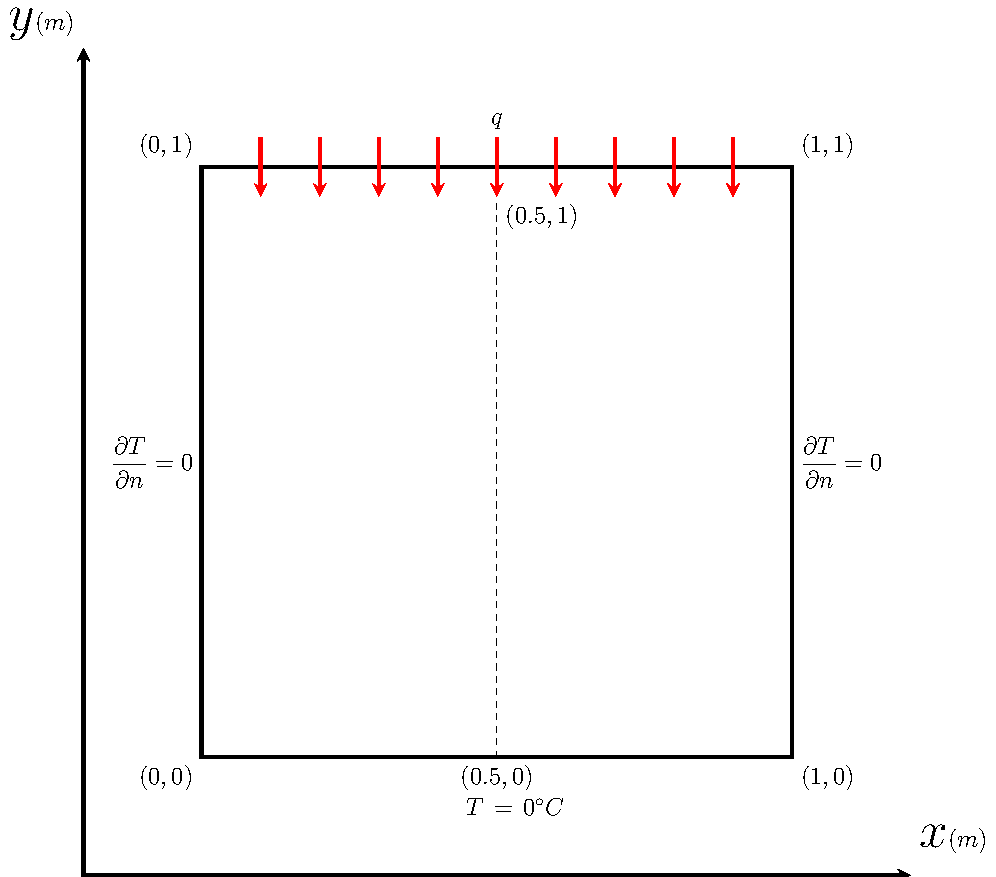
\includegraphics[width=.7\linewidth]{figures/poisson_neumann_boundary_conditions.pdf}
    \caption{Condições de contorno da placa para o problema de Poisson \ref{sec_poisson_neu}.}
    \label{poisson_n_bc}
\end{figure}

Novamente, foi utilizada uma malha triangular linear não estruturada com 768 elementos e 417 nós.
A \ref{poisson_n_3d} apresenta o campo de temperatura, onde os eixos $x$ e $y$ representam o dominio e o eixo $z$ é a distribuição de temperatura variando de 0 (cor azul) a 0.35 (vermelha).
\begin{figure}[H]
    \centering
    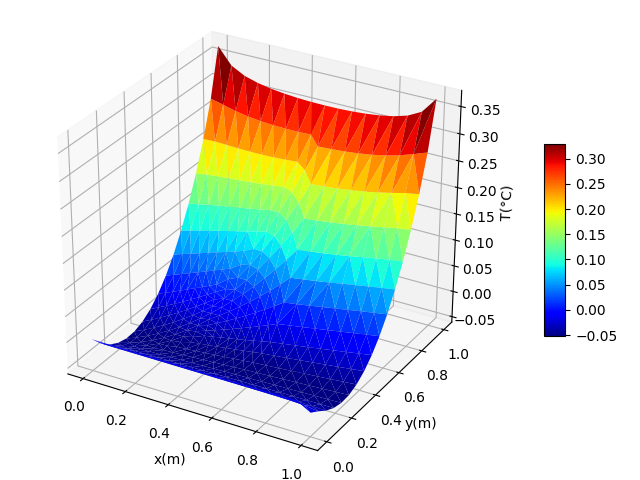
\includegraphics[width=.7\linewidth]{figures/poisson_neumann_permanent_3d.png}
    \caption{Distribuição de temperaturas na placa da solução do problema permanente de Poisson \ref{sec_poisson_neu}.}
    \label{poisson_n_3d}
\end{figure}

A comparação entre os resultados da solução analítica \eqref{poisson_n_sol} e a solução numérica, para a seção $x=0.5m$, é apresentada na \ref{poisson_n_perm_comp}, onde pode-se observar que ambas possuem o mesmo perfil.
A semelhança entre elas é quantificada pelo erro relativo médio que foi de $0.427\%$ e com desvio padrão de $0.8414\%$:
\begin{figure}[H]
    \centering
    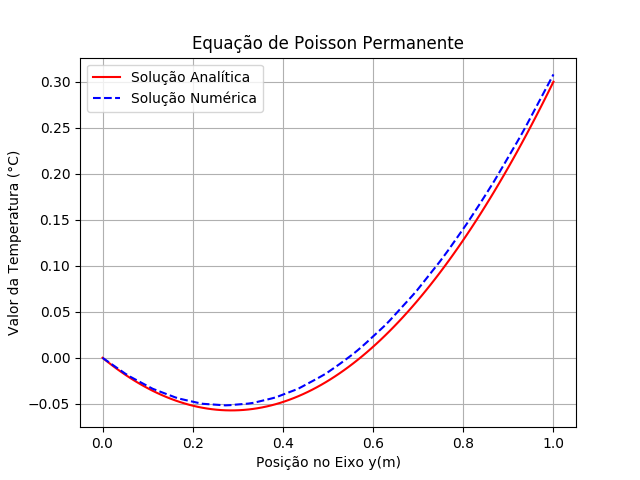
\includegraphics[width=.7\linewidth]{figures/poisson_neumann_permanent_comparison.png}
    \caption{Comparação de resultado das soluções númerica e analítica do problema de transporte de temperatura em sólidos no regime permanente com geração e fluxo de calor.}
    \label{poisson_n_perm_comp}
\end{figure}

As condições iniciais $t=0s$ atribuídas aos pontos sem condição de contorno foram de um valor inicial de $0^{\circ}C$.
A \ref{poisson_n_trans_comp} apresenta a evolução do campo de temperaturas em função do tempo.
É possível observar que a solução numérica converge para a solução analítica.
O erro relativo médio calculado para este caso foi de $0.31\%$ e com desvio padrão de $0.9205\%$.
\begin{figure}[H]
    \centering
    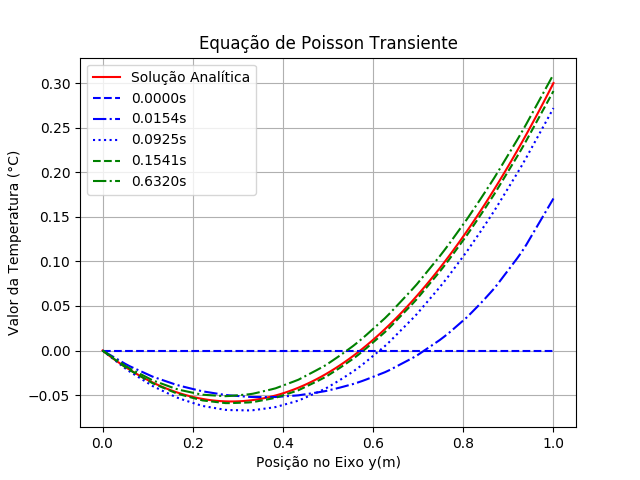
\includegraphics[width=.7\linewidth]{figures/poisson_neumann_transient_comparison.png}
    \caption{Comparação de resultado das soluções númerica e analítica do problema de transporte de temperatura em sólidos no regime permanente com geração e fluxo de calor.}
    \label{poisson_n_trans_comp}
\end{figure}

%---------------------------------------------------------------------------------------------Validação de fluidos
\section{\textbf{Validações de Problemas em Fluídos}}
\label{sec_fluidos}
%---------------------------------------------------------------------------------------------Primeiro Exemplo
\subsection{\textbf{Escoamento de Poiseuille}}
%---------------------------------------------------------------------------------------------Segundo Exemplo
\subsection{\textbf{Escoamento de Couette}}
%---------------------------------------------------------------------------------------------Terceiro Exemplo
\subsection{\textbf{Escoamento de Cavidade (\textit{Lid-Driven Cavity Flow})}}


%---------------------------------------------------------------------------------------------Validação de partículas
\section{\textbf{Validações de Problemas em Partículas}}
\label{sec_particulas}
%---------------------------------------------------------------------------------------------Primeiro Exemplo
\subsection{\textbf{Força Gravitacional}}

Mean Error: -7.706324287531013e-06
Standard Error: 1.7532532539087766e-05
%---------------------------------------------------------------------------------------------Segundo Exemplo
\subsection{\textbf{Força de Arrasto}}

Mean Error: 3.083075647620123e-07
Standard Error: 1.6723400282002147e-07
%---------------------------------------------------------------------------------------------Terceiro Exemplo
\subsection{\textbf{Força de Sustentação}}

Mean Error: 6.52554446290127e-08
Standard Error: 3.79349081853567e-08

%---------------------------------------------------------------------------------------------Terceiro Exemplo
\subsection{\textbf{Força de Massa Virtual (\textit{Added Mass})}}

Mean Error: -6.657465890493951e-05
Standard Error: 1.1362509215219308e-05